\chapter{Evaluation}
\label{cha:evaluation}
In this chapter we present the evaluation of the work done. This will measure the performance and scalability of the integration by presenting benchmarks of the running system.\par
	Section \ref{sec:operation_propagation_time} will measure how the number of operation each message contains influences the time needed to propagate them. In section \ref{sec:meta-data_size} will be shown how the meta-data stored in Antidote increases with the operations executed in the system.

\section{Operation Propagation Time}
\label{sec:operation_propagation_time}
In this section we will focus on measuring the propagation time of system operations and how it fluctuates with other variables. In this test scenario, we use one Antidote instance, one legion object server instance, one Antidote client and one Legion node. All the system components are located in the same network. This experiment consists in saving the current time in one client, when the update is issued. The update is sent and when the other client detects to have received the update, saves the time and finally makes the difference between the two times.\par
	Firstly, in figure \ref{graph1} we measure the operation propagation time scaling with the number of operations in each message. As we can see, the time it takes to propagate a message, increases with the number of operations that each message contains. When propagating messages from Legion to Antidote, the time required increases nearly linearly with the number of operations. On the other hand, when propagating messages from Antidote to legion, the time required does not grow as fast, only increasing slightly with the number of operations in each message.

\begin{figure}[H]
\centering
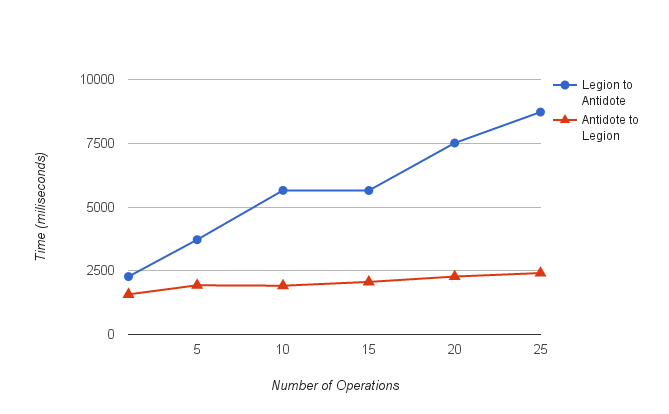
\includegraphics[scale=0.7]{files/graph1.png}
\caption{Propagation time scaling with operations per message}
\label{graph1}
\end{figure}

\begin{figure}[h]
\centering
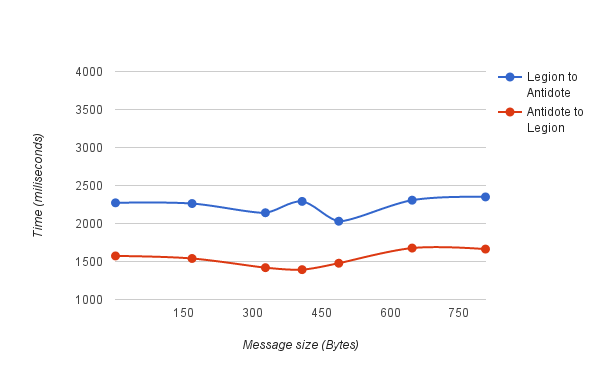
\includegraphics[scale=0.7]{files/chart2.png}
\caption{Propagation time scaling with message size}
\label{chart2}
\end{figure}

Secondly, in \ref{chart2} we  measure the scalability of the message propagation time with the size of the message. As we can see, the time needed to propagate a message does not seem to scale with the size of the message. Although the updates from Antidote to Legion still propagate faster, both update directions are not influenced by the size of the message, resulting in a chart with fluctuating time values and no growing pattern.

\section{Meta-Data Size}
\label{sec:meta-data_size}
As explained in \ref{sec:proxy_development}, in order to keep the system from propagating duplicated operations, there is a need to store meta-data information in the Antidote nodes. In this section we measure the size of this meta-data along with it's scalability as the system runs. The measured values in figure \ref{chart3} are a representation of the size of meta-data stored in an Antidote node. In this test scenario, we consider write and delete operations, as these separately will influence the final size of meta-data. The blue line represents a workload where 50\% of the updates are writes and the other 50\% are deletes. On the other hand, the red line has a more write intensive workload, with 80\% writes and 20\% deletes.\par
	As expected, the meta-data size stored increases with the number of operations. In the red workload, the growing is continuously linear. The blue workload also grows continuously, but needs less memory. This is due to the unique tokens that are erased when a delete operation is issued, making the only stored data the operation identifiers.\par
	The always growing tendency of the meta-data derives from the operation identifiers that will keep stacking as the system runs. This points the lack of a garbage collector in order to clean the no longer needed operation identifiers from time to time.

\begin{figure}[h]
\centering
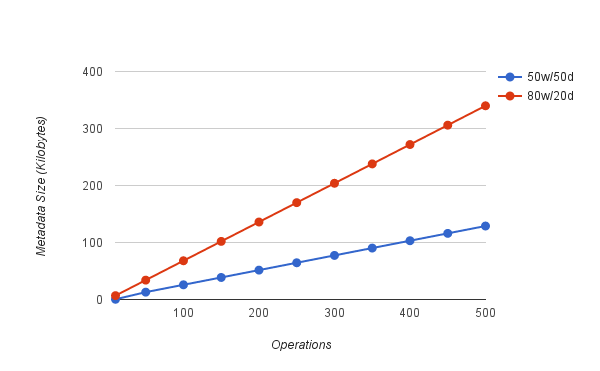
\includegraphics[scale=0.7]{files/chart3.png}
\caption{Meta-data size scaling with propagated operations}
\label{chart3}
\end{figure}